\documentclass[sigconf,edbt]{acmart-edbt2021}

\def\BibTeX{{\rm B\kern-.05em{\sc i\kern-.025em b}\kern-.08em
    T\kern-.1667em\lower.7ex\hbox{E}\kern-.125emX}}

\usepackage{booktabs} % For formal tables


% Copyright
\setcopyright{rightsretained}

% DOI
\acmDOI{}

% ISBN
\acmISBN{XXXXXXXX}

%Conference
\acmConference[EDBT 2021]{24th International Conference on Extending Database Technology (EDBT)}{March 23-26, 2021}{Nicosia, Cyprus} 
\acmYear{2021}

\settopmatter{printacmref=false, printccs=false, printfolios=false}

\pagestyle{empty} % removes running headers

\begin{document}
\title{ContextFree Wars: The RedisGraph Strikes Back}
% \begin{document}
% \title{Implementing support for context-free path queering for the Cypher extension in RedisGraph}
% \titlenote{Produces the permission block, and copyright information}
% \subtitle{Extended Abstract}
% \subtitlenote{The full version of the author's guide is available as
%   \texttt{acmart.pdf} document}
  

\author{Semyon Grigorev}
	\email{s.v.grigoriev@spbu.ru}
	\email{semyon.grigorev@jetbrains.com}
	\orcid{0000-0002-7966-0698}
	\affiliation{
		\institution{Saint Petersburg State University}
		\streetaddress{7/9 Universitetskaya nab.}
		\city{St. Petersburg}
		\country{Russia}
		\postcode{199034}
	}
	\affiliation{
		\institution{JetBrains Research}
		\streetaddress{Primorskiy prospekt 68-70, Building 1}
		\city{St. Petersburg}
		\country{Russia}
		\postcode{199034}
	}

\author{Arseniy Terekhov}
	\email{simpletondl@yandex.ru}
	\affiliation{%
		\institution{Saint Petersburg State University}
		\streetaddress{7/9 Universitetskaya nab.}
		\city{St. Petersburg}
		\country{Russia}
		\postcode{199034}
	}
% The default list of authors is too long for headers}
% \renewcommand{\shortauthors}{B. Trovato et al.}
\renewcommand{\shortauthors}{}


\begin{abstract}
A long time ago in a galaxy far far away...
\end{abstract}

%
% % The code below should be generated by the tool at
% % http://dl.acm.org/ccs.cfm
% % Please copy and paste the code instead of the example below. 
% %
% \begin{CCSXML}
% <ccs2012>
%  <concept>
%   <concept_id>10010520.10010553.10010562</concept_id>
%   <concept_desc>Computer systems organization~Embedded systems</concept_desc>
%   <concept_significance>500</concept_significance>
%  </concept>
%  <concept>
%   <concept_id>10010520.10010575.10010755</concept_id>
%   <concept_desc>Computer systems organization~Redundancy</concept_desc>
%   <concept_significance>300</concept_significance>
%  </concept>
%  <concept>
%   <concept_id>10010520.10010553.10010554</concept_id>
%   <concept_desc>Computer systems organization~Robotics</concept_desc>
%   <concept_significance>100</concept_significance>
%  </concept>
%  <concept>
%   <concept_id>10003033.10003083.10003095</concept_id>
%   <concept_desc>Networks~Network reliability</concept_desc>
%   <concept_significance>100</concept_significance>
%  </concept>
% </ccs2012>  
% \end{CCSXML}
% 
% \ccsdesc[500]{Computer systems organization~Embedded systems}
% \ccsdesc[300]{Computer systems organization~Redundancy}
% \ccsdesc{Computer systems organization~Robotics}
% \ccsdesc[100]{Networks~Network reliability}


% \keywords{ACM proceedings, \LaTeX, text tagging}

%% A "teaser" image appears between the author and affiliation
%% information and the body of the document, and typically spans the
%% page.
\begin{teaserfigure}
  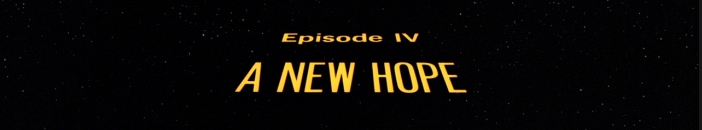
\includegraphics[width=\textwidth]{new_hope.png}
  \caption{Episode IV: A New Hope}
  \label{fig:teaser}
\end{teaserfigure}

\maketitle

\input{samplebody-conf}

%%
%% The next two lines define the bibliography style to be used, and
%% the bibliography file.
\bibliographystyle{ACM-Reference-Format}
\bibliography{sample-base}

%%
%% If your work has an appendix, this is the place to put it.
%% Please note that all the content must fit within the page limits, including any appendices.
%\appendix
%
%\section{Research Methods}
% ...

\end{document}
\endinput
